\section{Estudio de Calidad de Imagen}

En esta seccion se estudiaron configuraciones que afectan la calidad de imagen resultante. Para el estudio de diferencia entre imagenes se utilizo el software PerceptualDiff basado en el trabajo de Hector Yee y otros en 2001 \cite{Yee:2001:SSV:383745.383748}, este nos permite detectar la diferencia perceptual entre dos imagenes.

\subsection{Composicion Final de Imagen}
Todas las imagenes en esta seccion fueron renderizadas con una resolucion de pantalla de $1920x1080$, con una resolucion para la representacion de voxeles de $512^3$ y con una longitud de marcha del cono de $0.5$. La representacion de voxeles solo contiene iluminacion directa.

\begin{figure}[H]
	\centering
	\begin{subfigure}[t]{.49\linewidth}
		\centering
		\captionsetup{justification=centering}
		\caption*{Directa}
		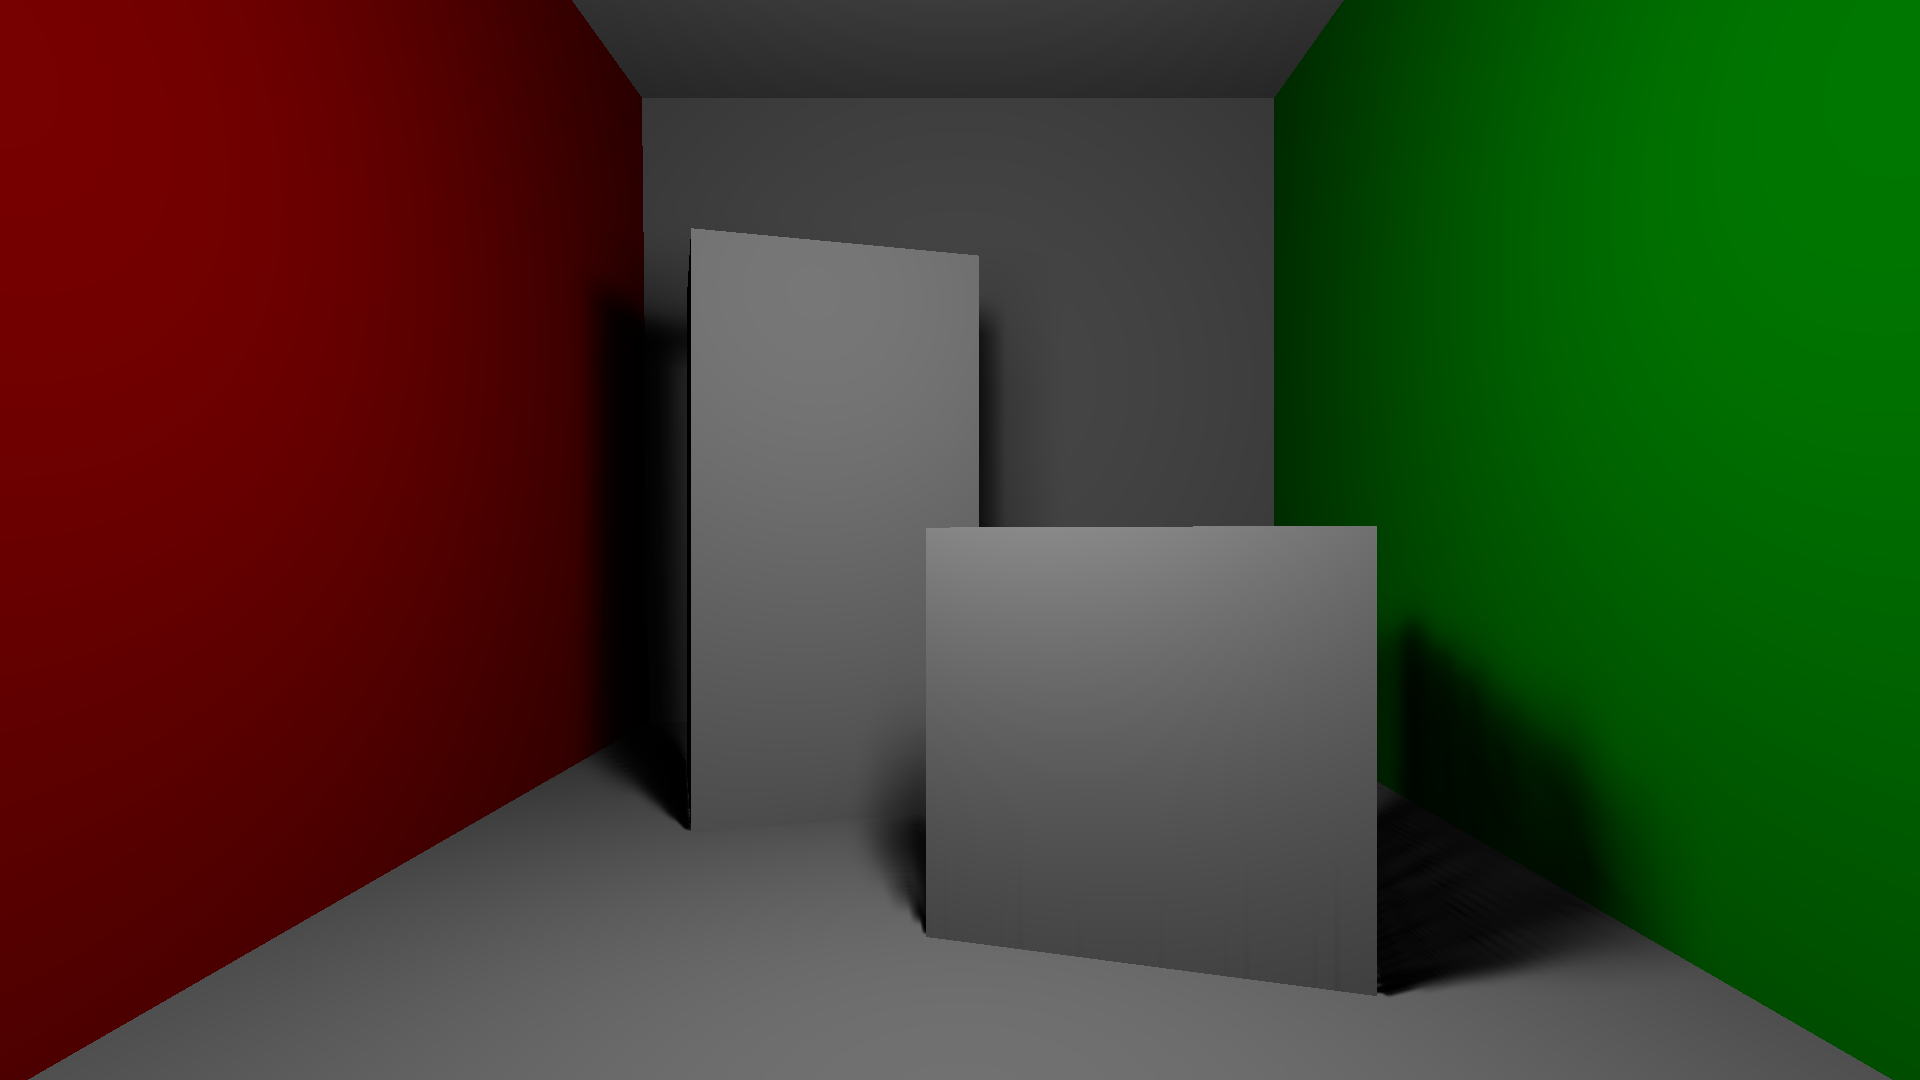
\includegraphics[width=\linewidth]{media/finals/cornell_direct.png}
	\end{subfigure}%
	\hspace{0.01\textwidth}
	\begin{subfigure}[t]{.49\linewidth}
		\centering
		\caption*{Indirecta}
		\captionsetup{justification=centering}
		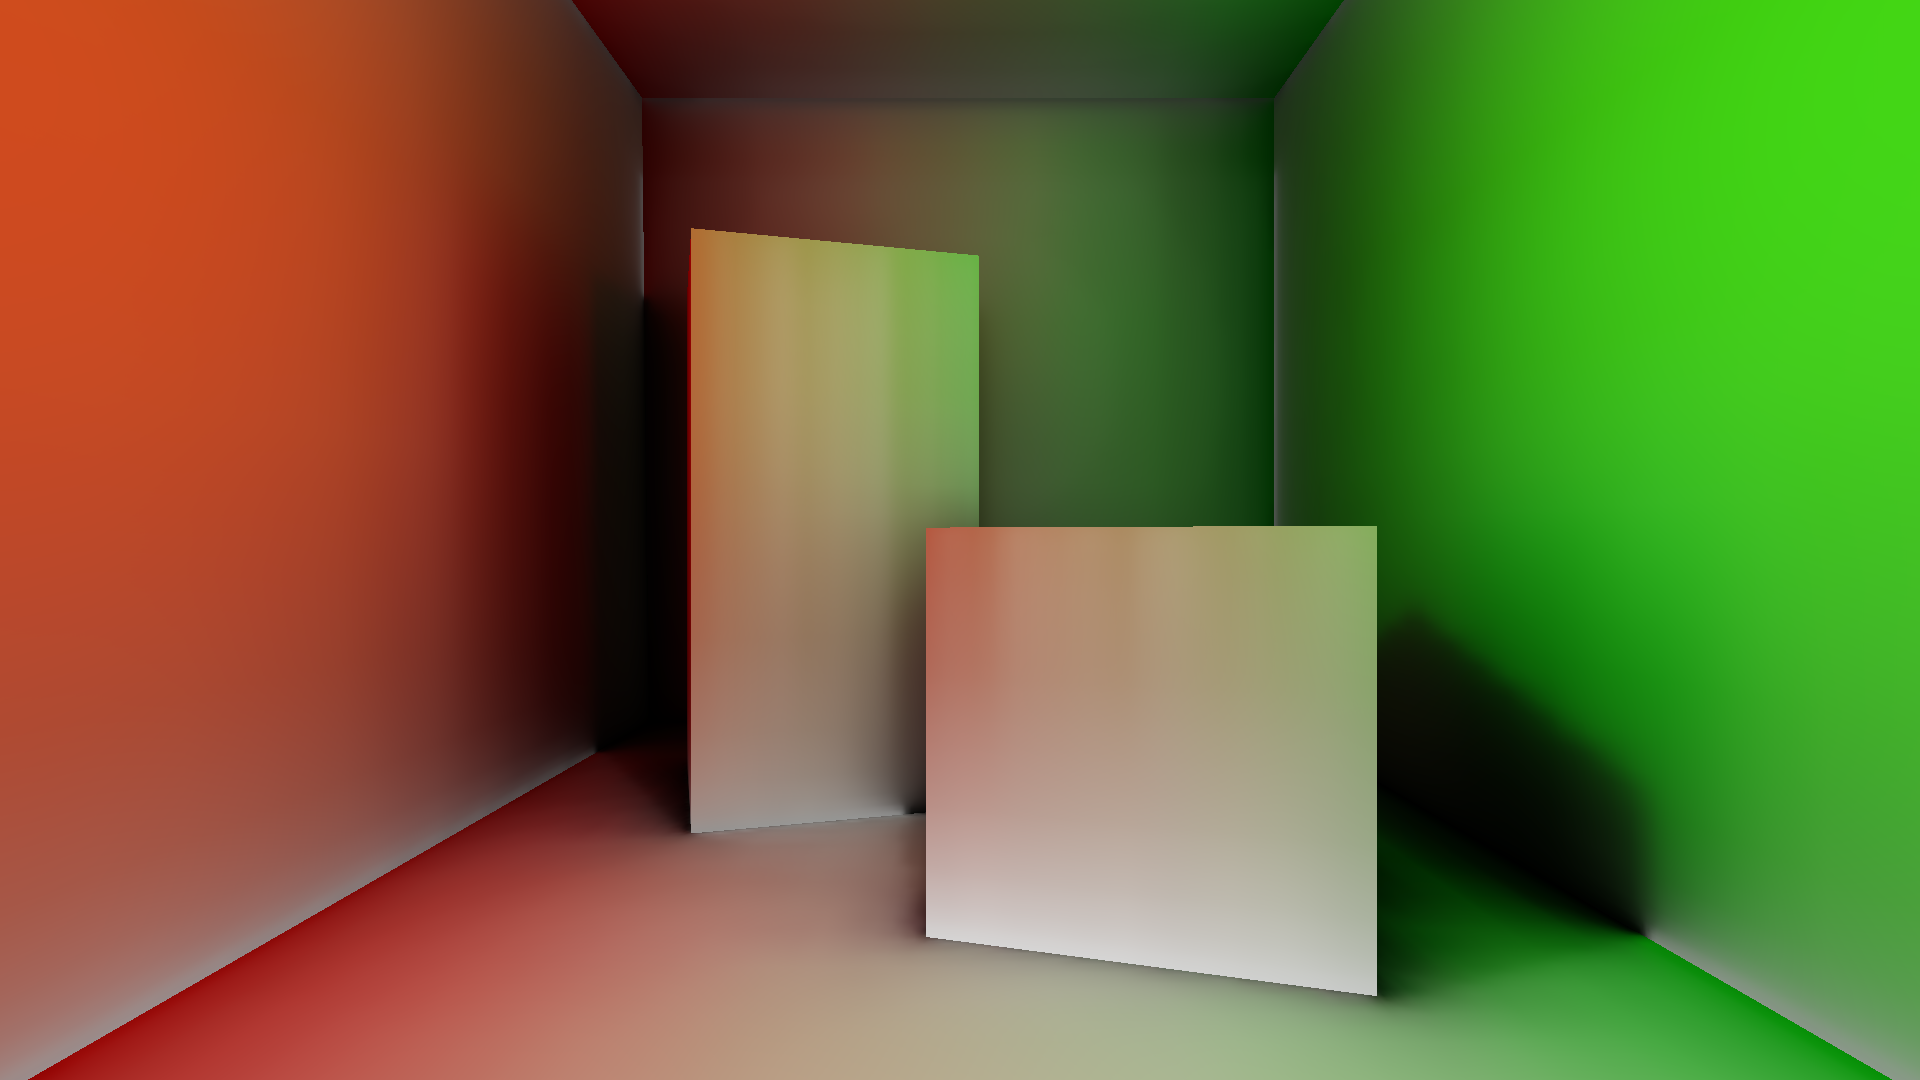
\includegraphics[width=\linewidth]{media/finals/cornell_indirect.png}
	\end{subfigure}%
	\par\bigskip
	\begin{subfigure}[t]{.49\linewidth}
		\centering
		\captionsetup{justification=centering}
		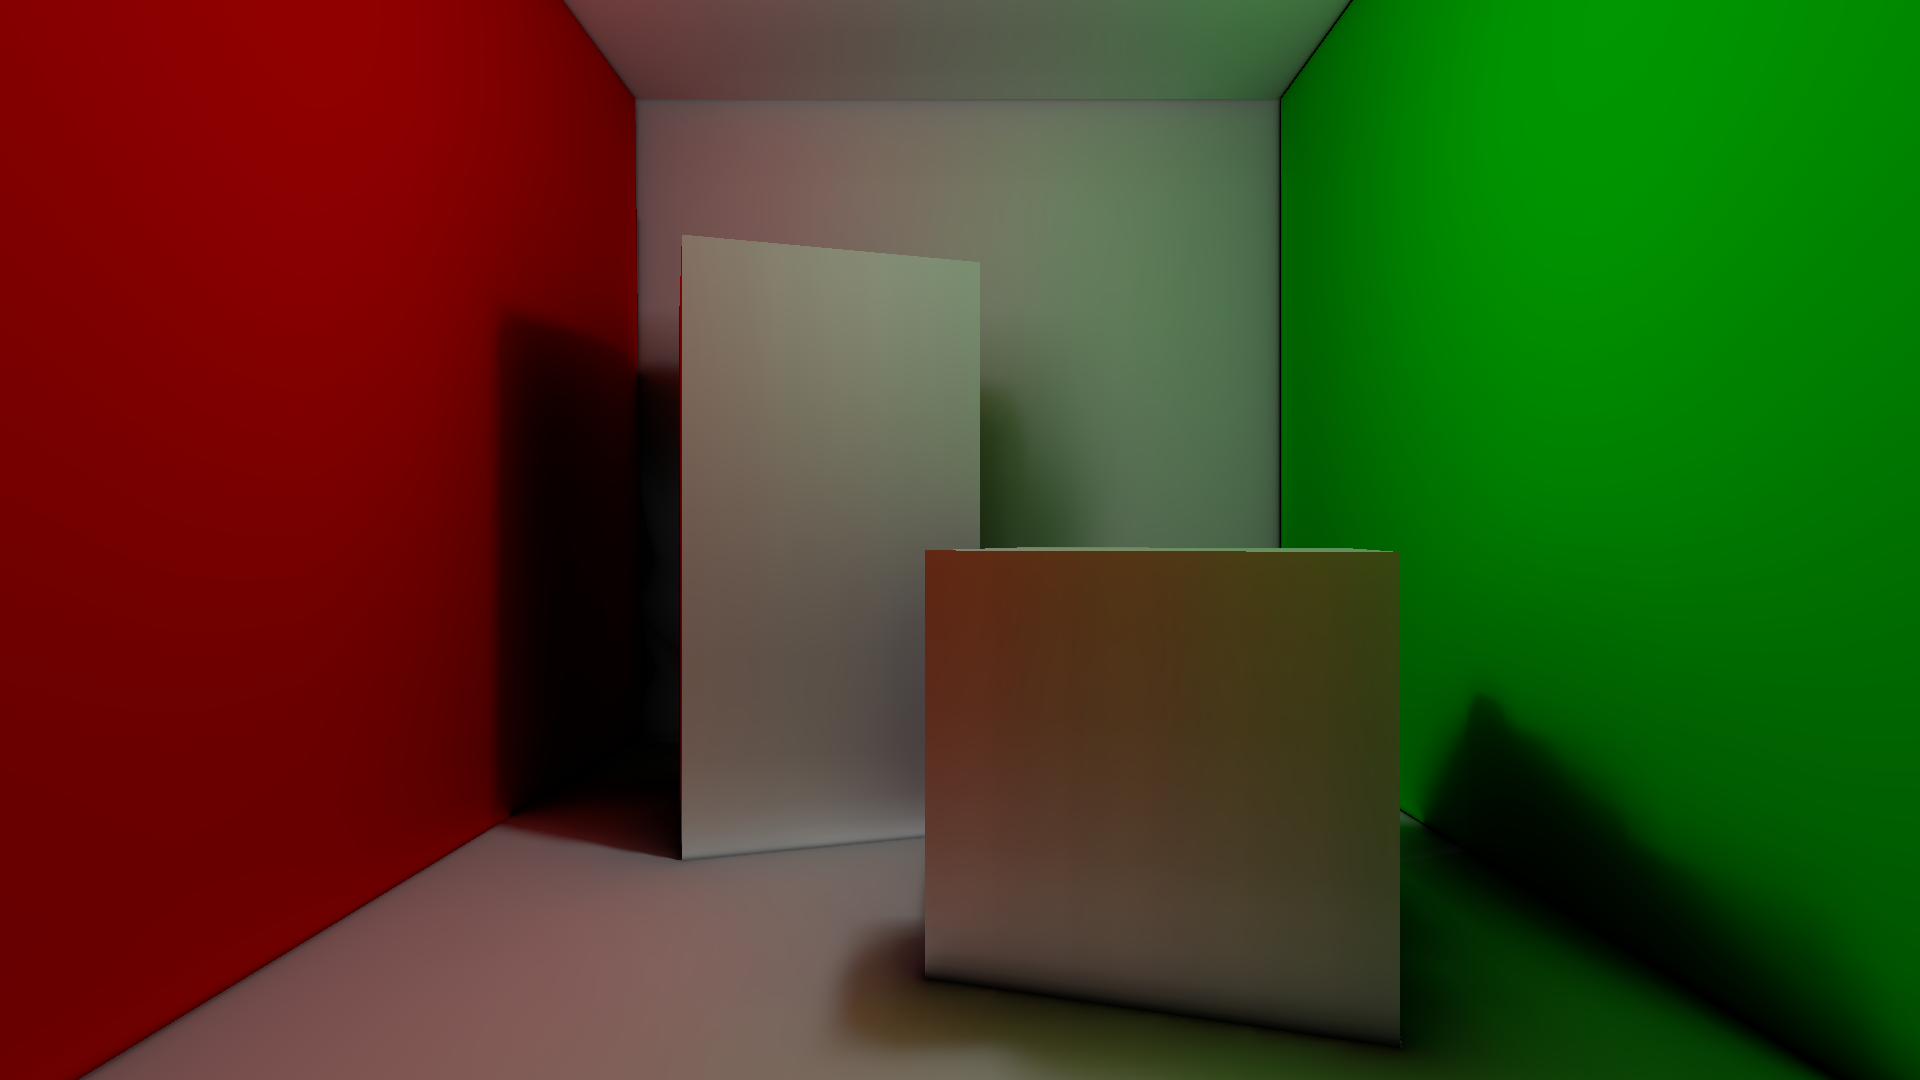
\includegraphics[width=\linewidth]{media/finals/cornell_gi.png}
		\caption*{Directa + Indirecta + Oclusion Ambiental}
	\end{subfigure}%
	\hspace{0.01\textwidth}
	\begin{subfigure}[t]{.49\linewidth}
		\centering
		\captionsetup{justification=centering}
		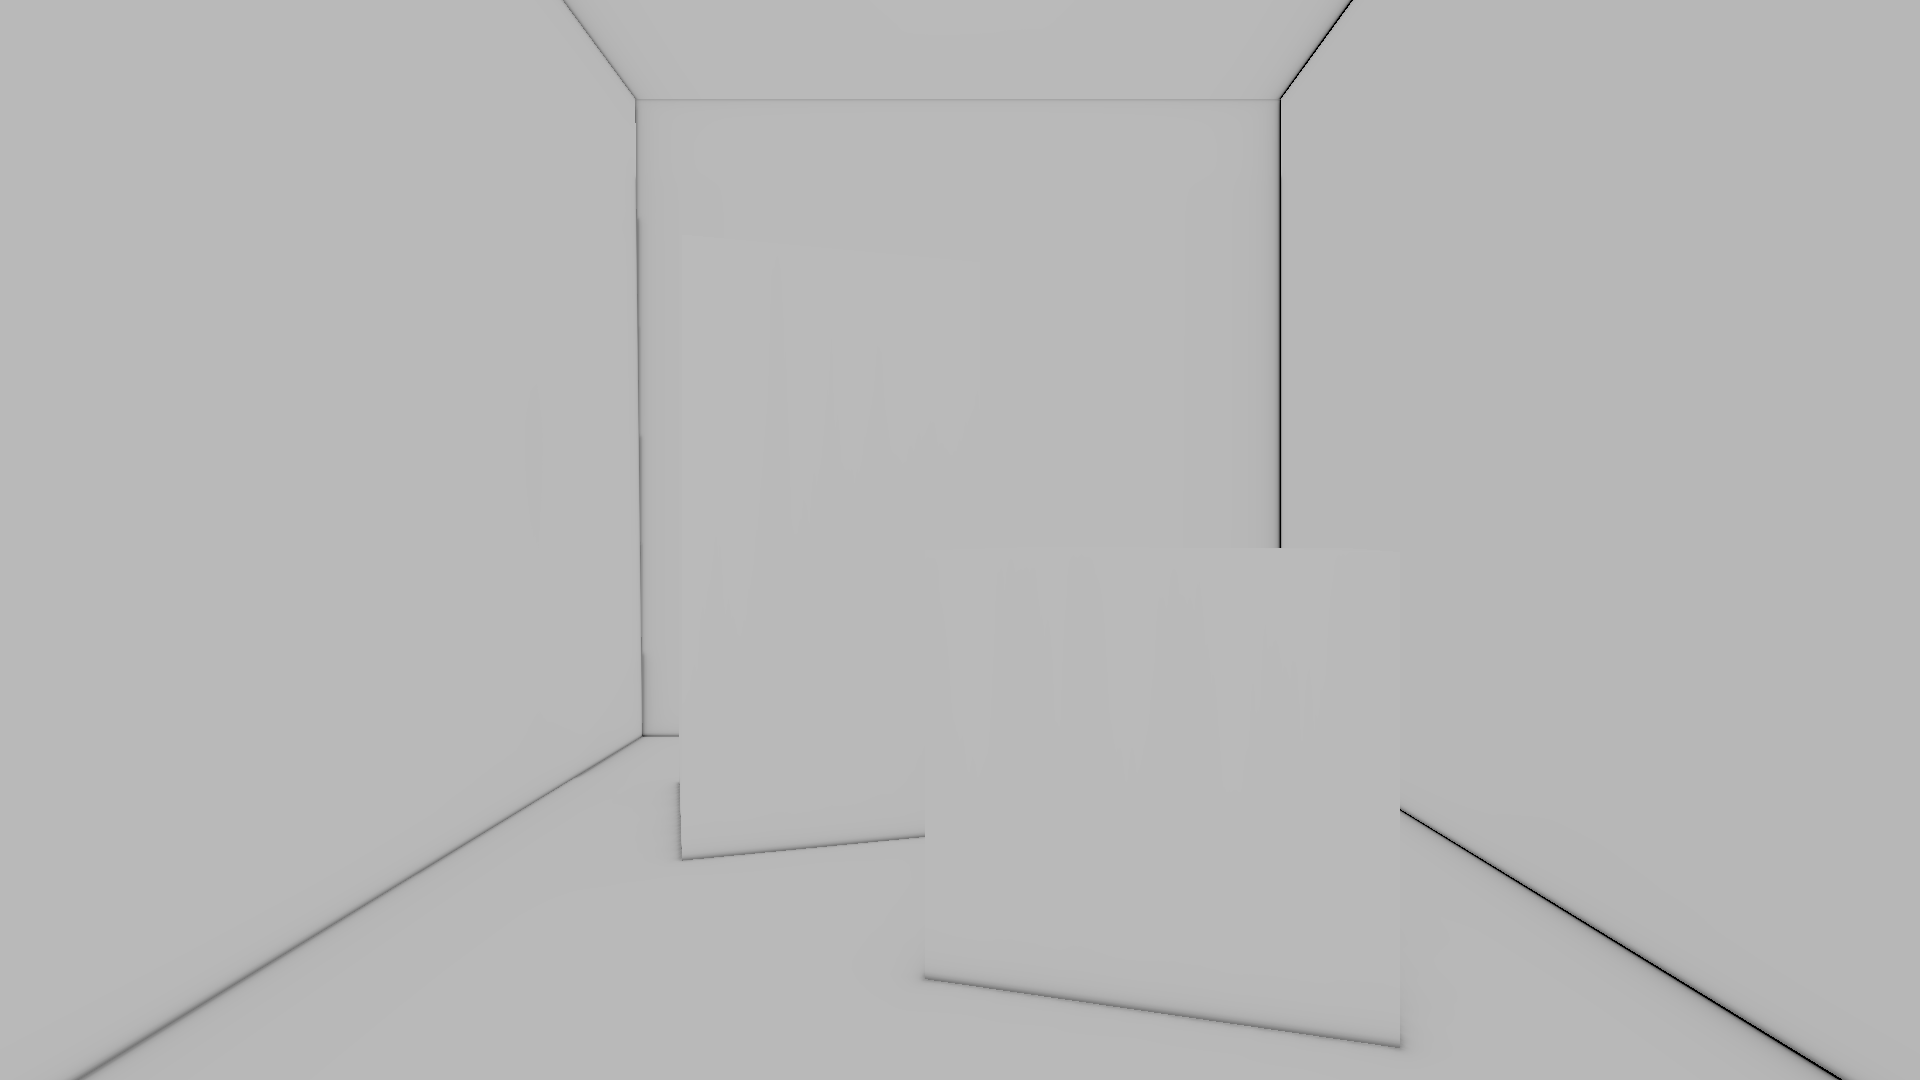
\includegraphics[width=\linewidth]{media/finals/cornell_ao.png}
		\caption*{Oclusion Ambiental}
	\end{subfigure}%
	\caption{Composicion para la escena Cornell Box.}
	\label{fig:cornell_final}
\end{figure}

\begin{figure}[H]
	\centering
	\begin{subfigure}[t]{.49\linewidth}
		\centering
		\captionsetup{justification=centering}
		% \caption*{Directa}
		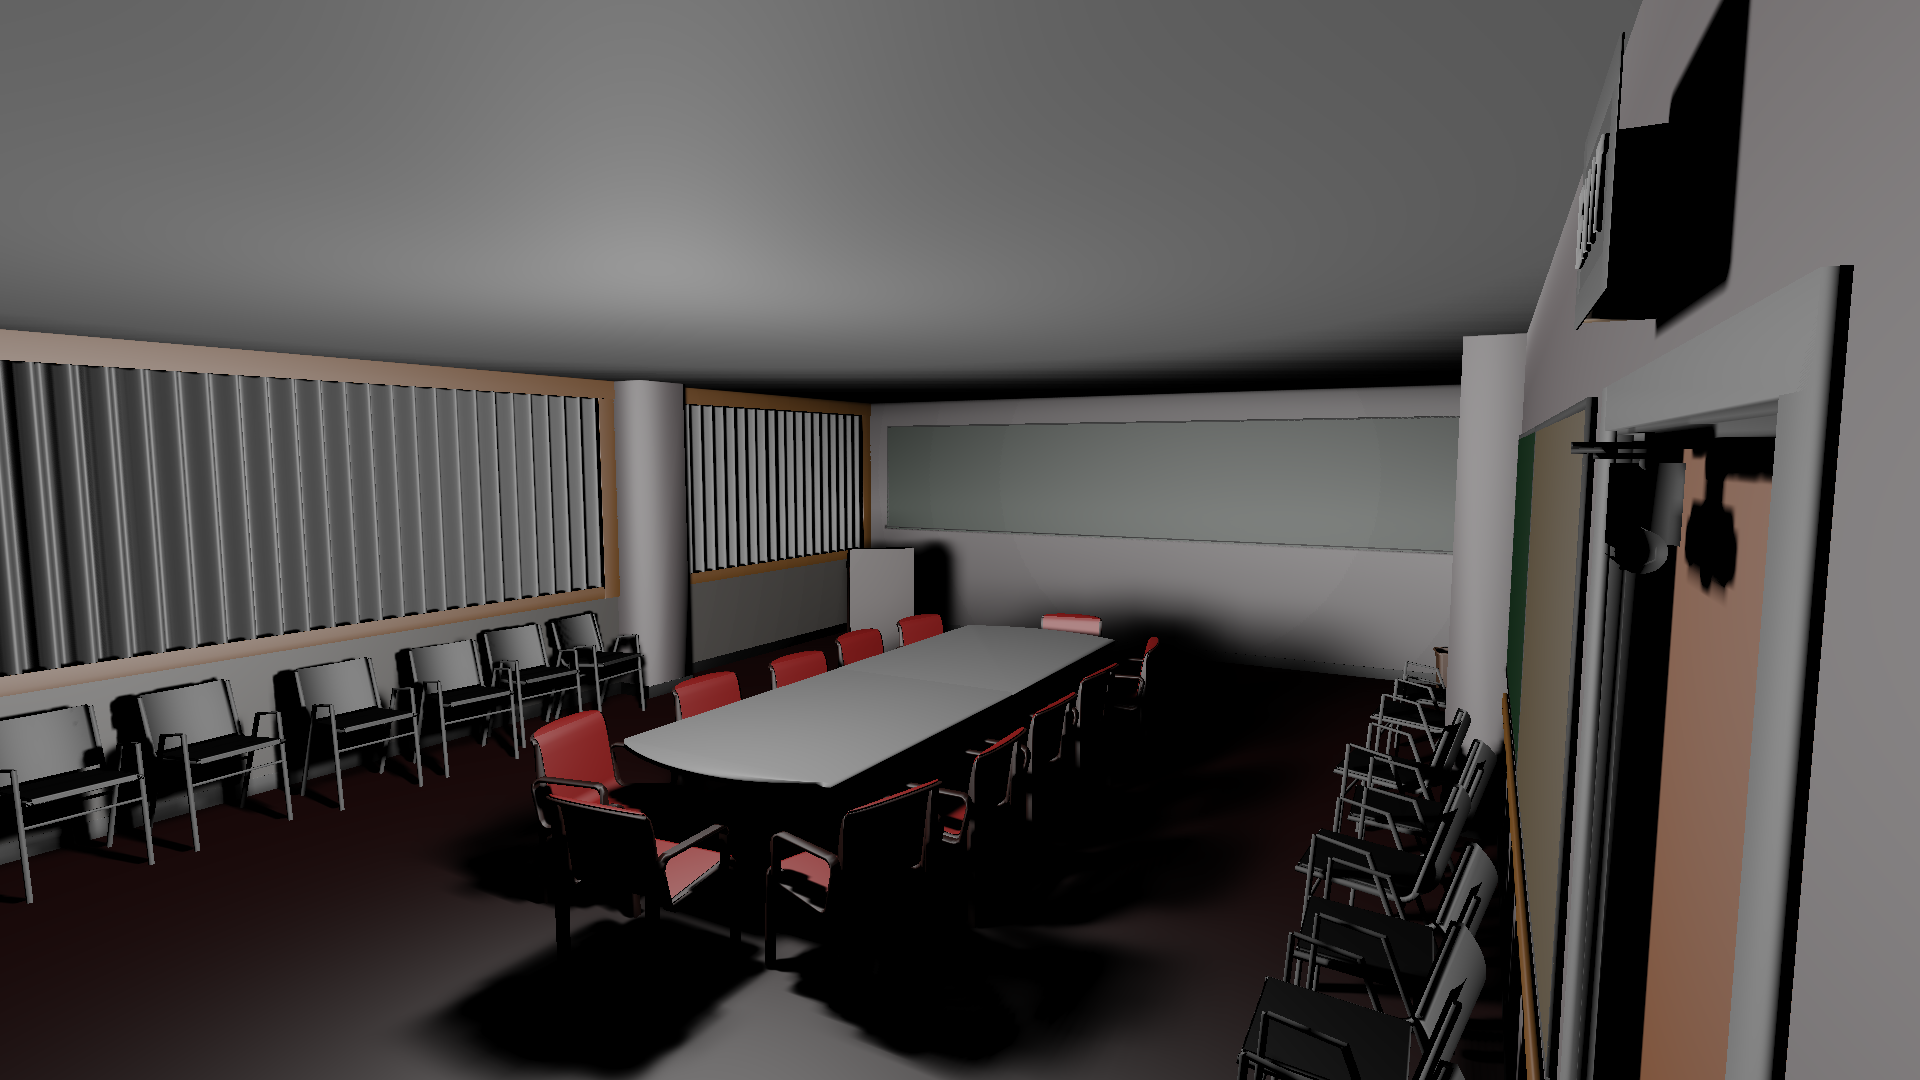
\includegraphics[width=\linewidth]{media/finals/conf_direct.png}
	\end{subfigure}%
	\hspace{0.01\textwidth}
	\begin{subfigure}[t]{.49\linewidth}
		\centering
		% \caption*{Indirecta}
		\captionsetup{justification=centering}
		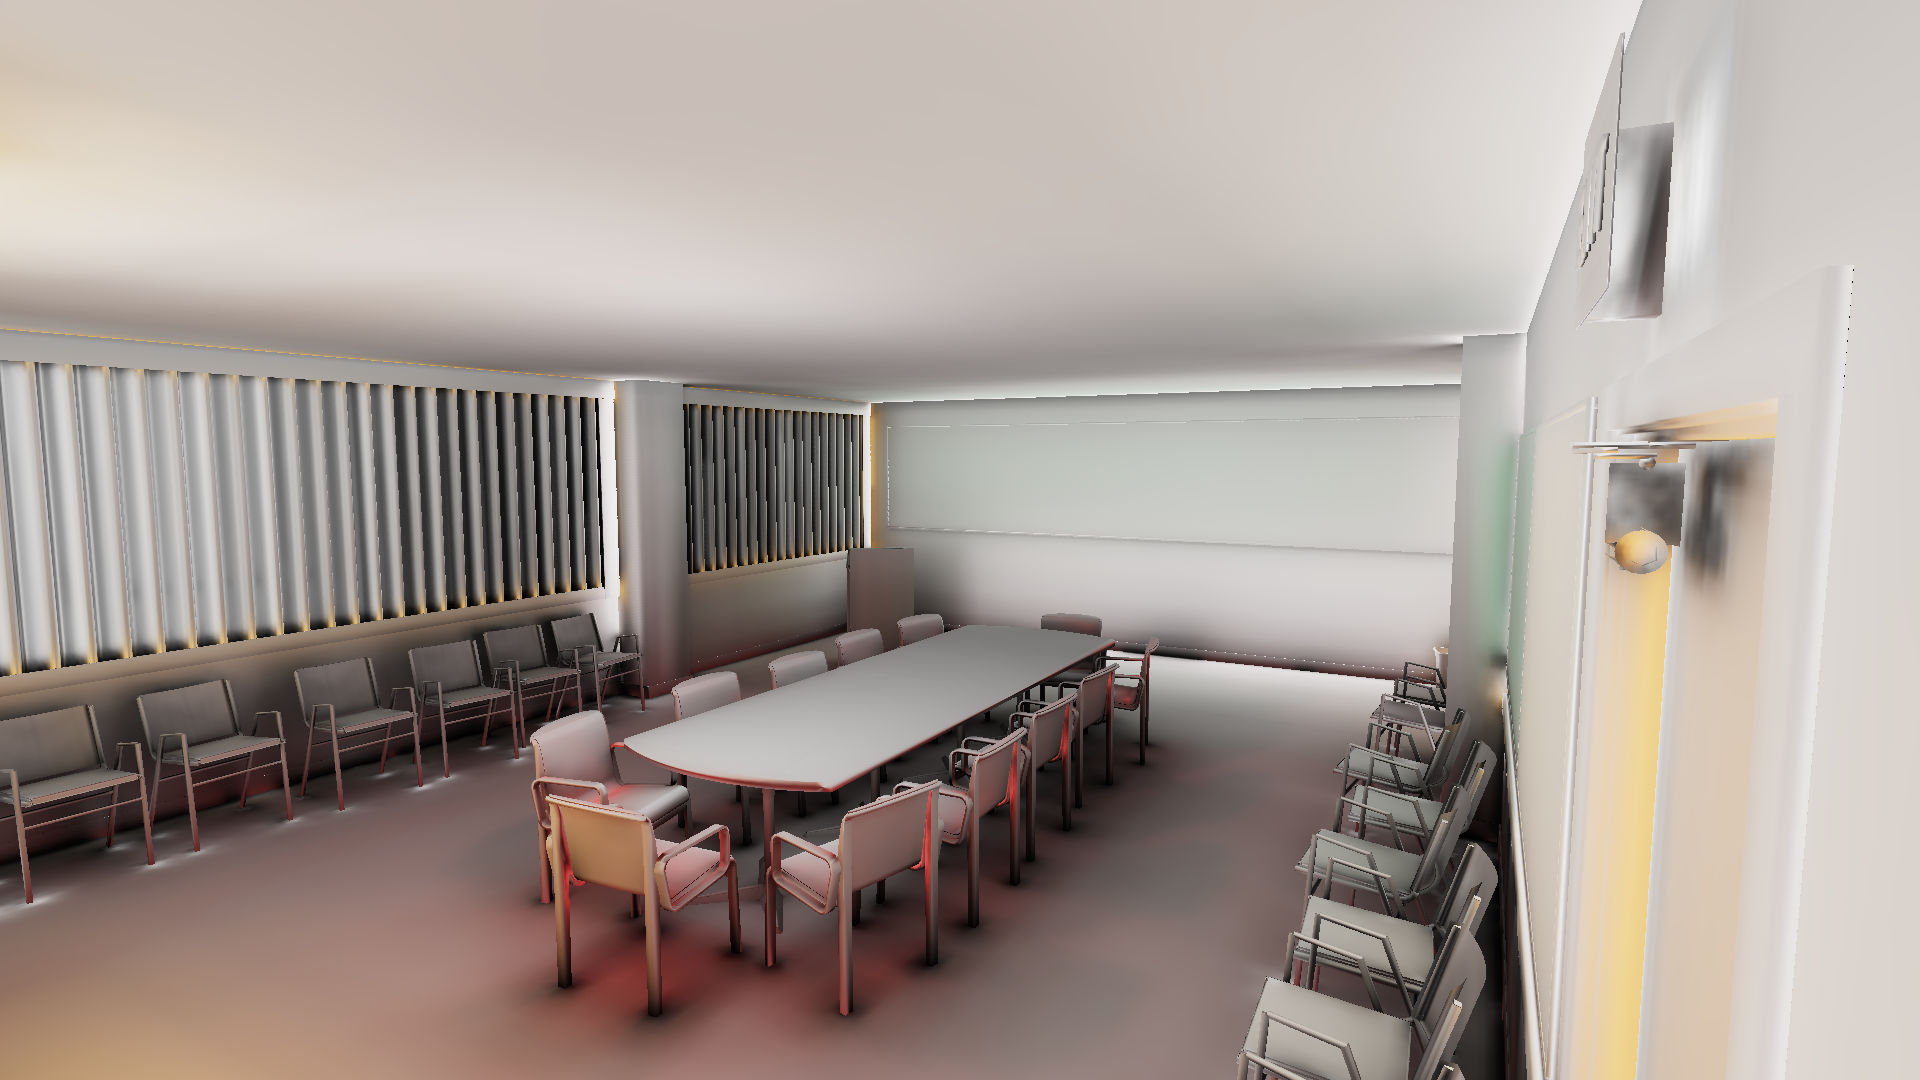
\includegraphics[width=\linewidth]{media/finals/conf_indirect.png}
	\end{subfigure}%
	\par\bigskip
	\begin{subfigure}[t]{.49\linewidth}
		\centering
		% \caption*{Directa + Indirecta + Oclusion Ambiental}
		\captionsetup{justification=centering}
		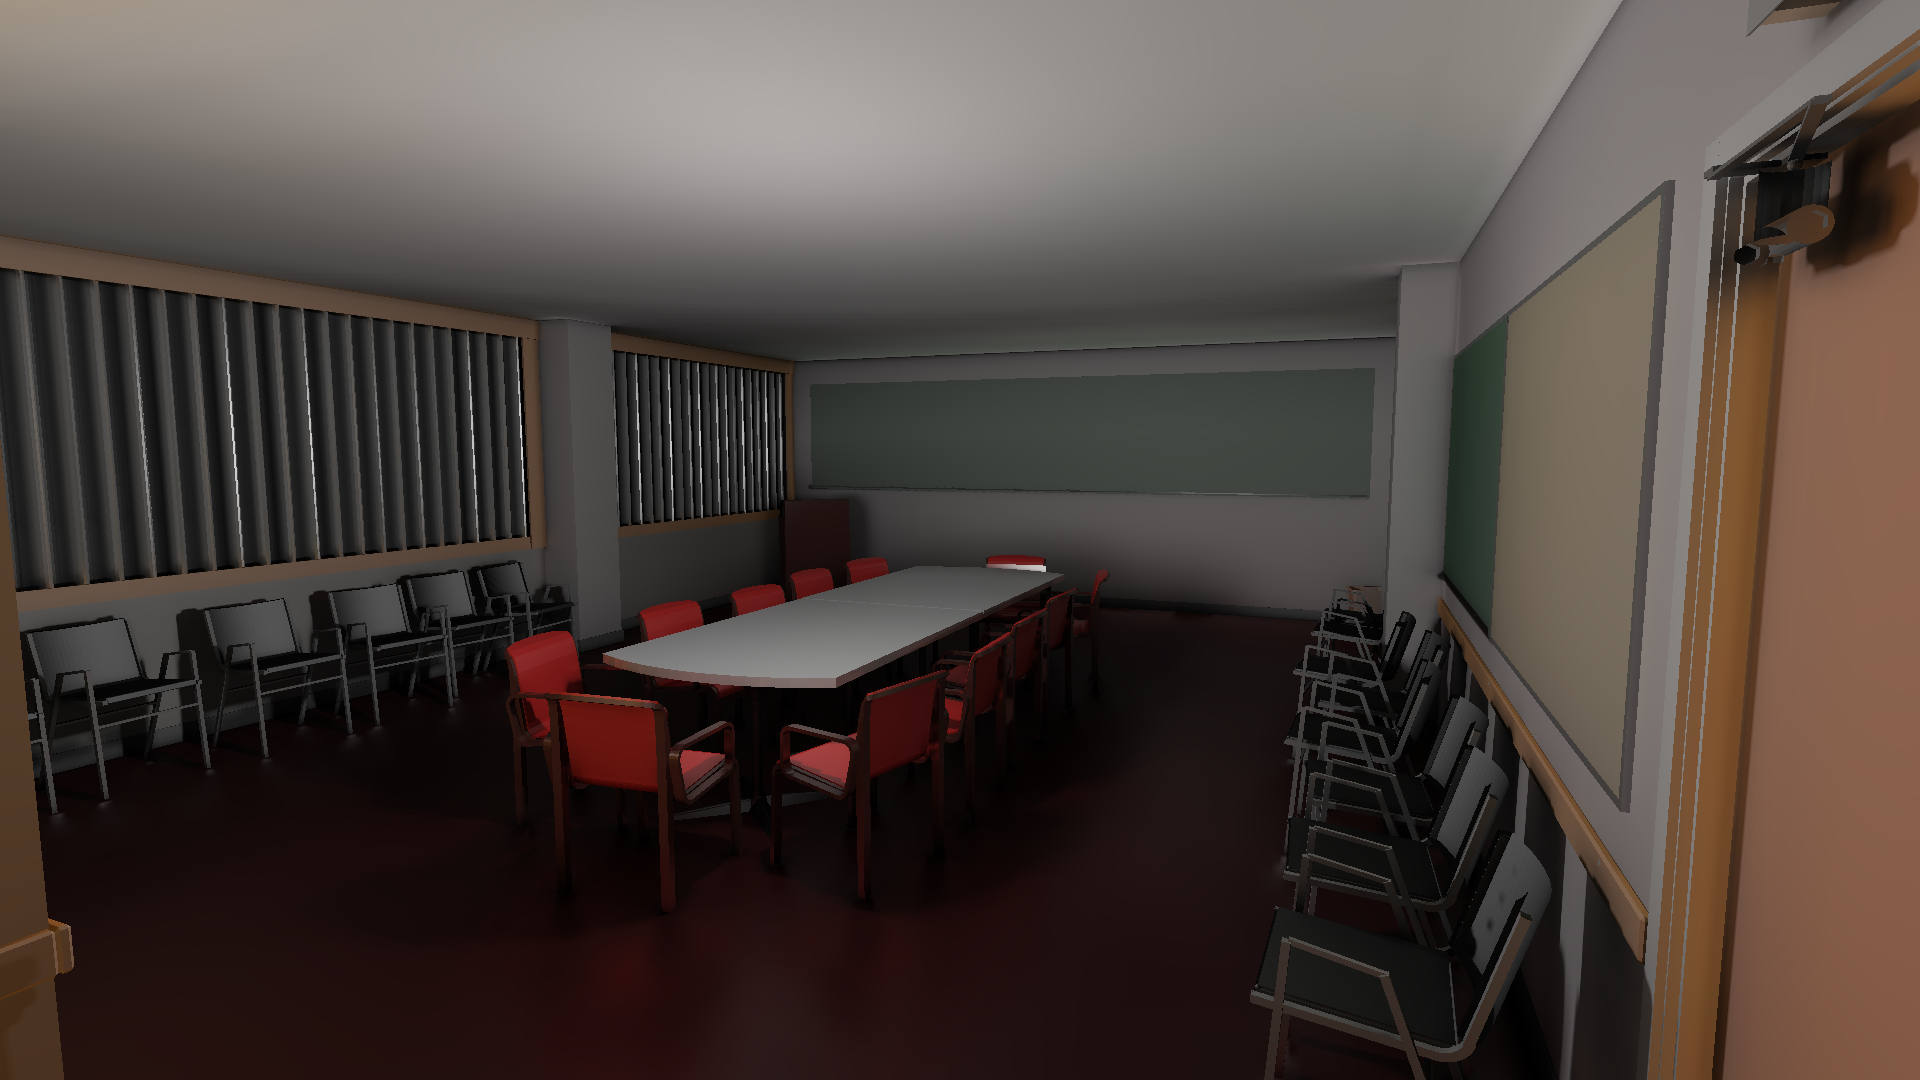
\includegraphics[width=\linewidth]{media/finals/conf_gi.png}
	\end{subfigure}%
	\hspace{0.01\textwidth}
	\begin{subfigure}[t]{.49\linewidth}
		\centering
		% \caption*{Oclusion Ambiental}
		\captionsetup{justification=centering}
		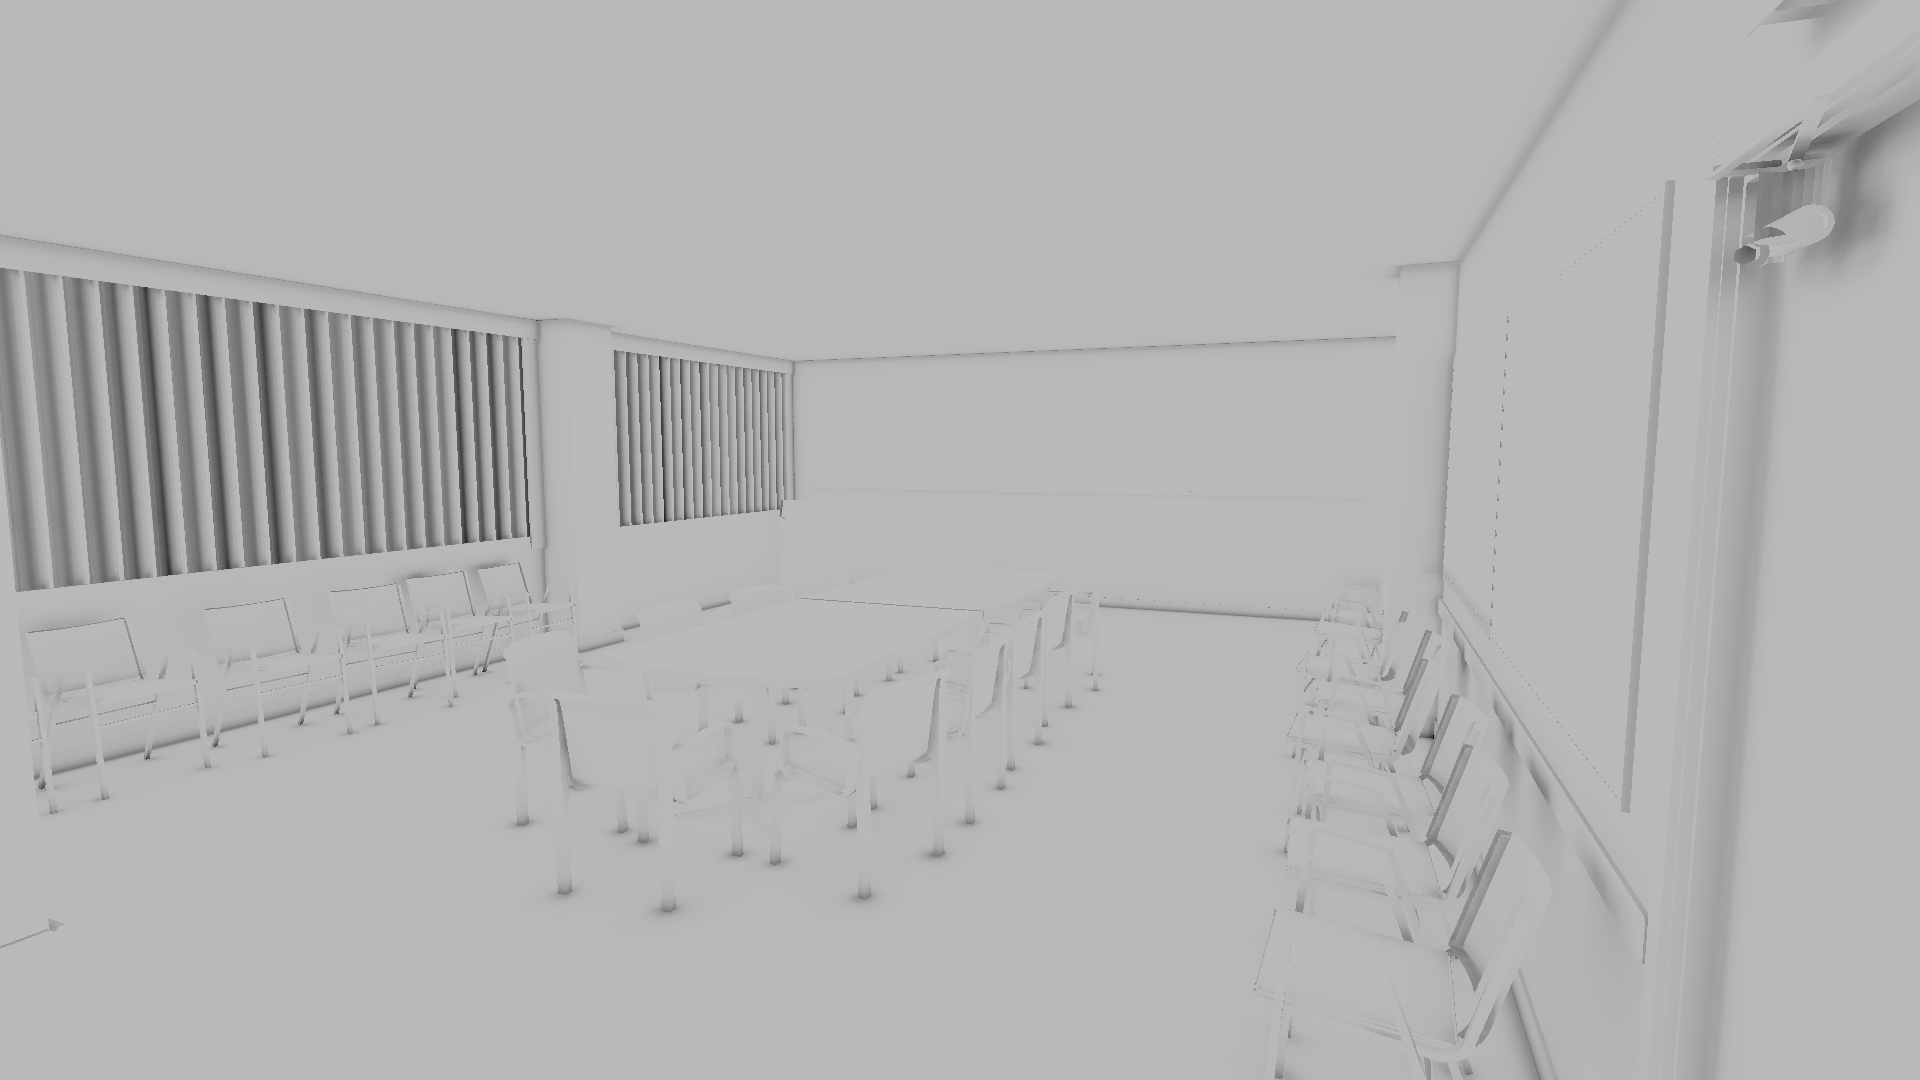
\includegraphics[width=\linewidth]{media/finals/conf_ao.png}
	\end{subfigure}%
	\caption{Composicion para la escena Conference.}
	\label{fig:conf_final}
\end{figure}
\begin{figure}[H]
	\centering
	\begin{subfigure}[t]{.49\linewidth}
		\centering
		\captionsetup{justification=centering}
		% \caption*{Directa}
		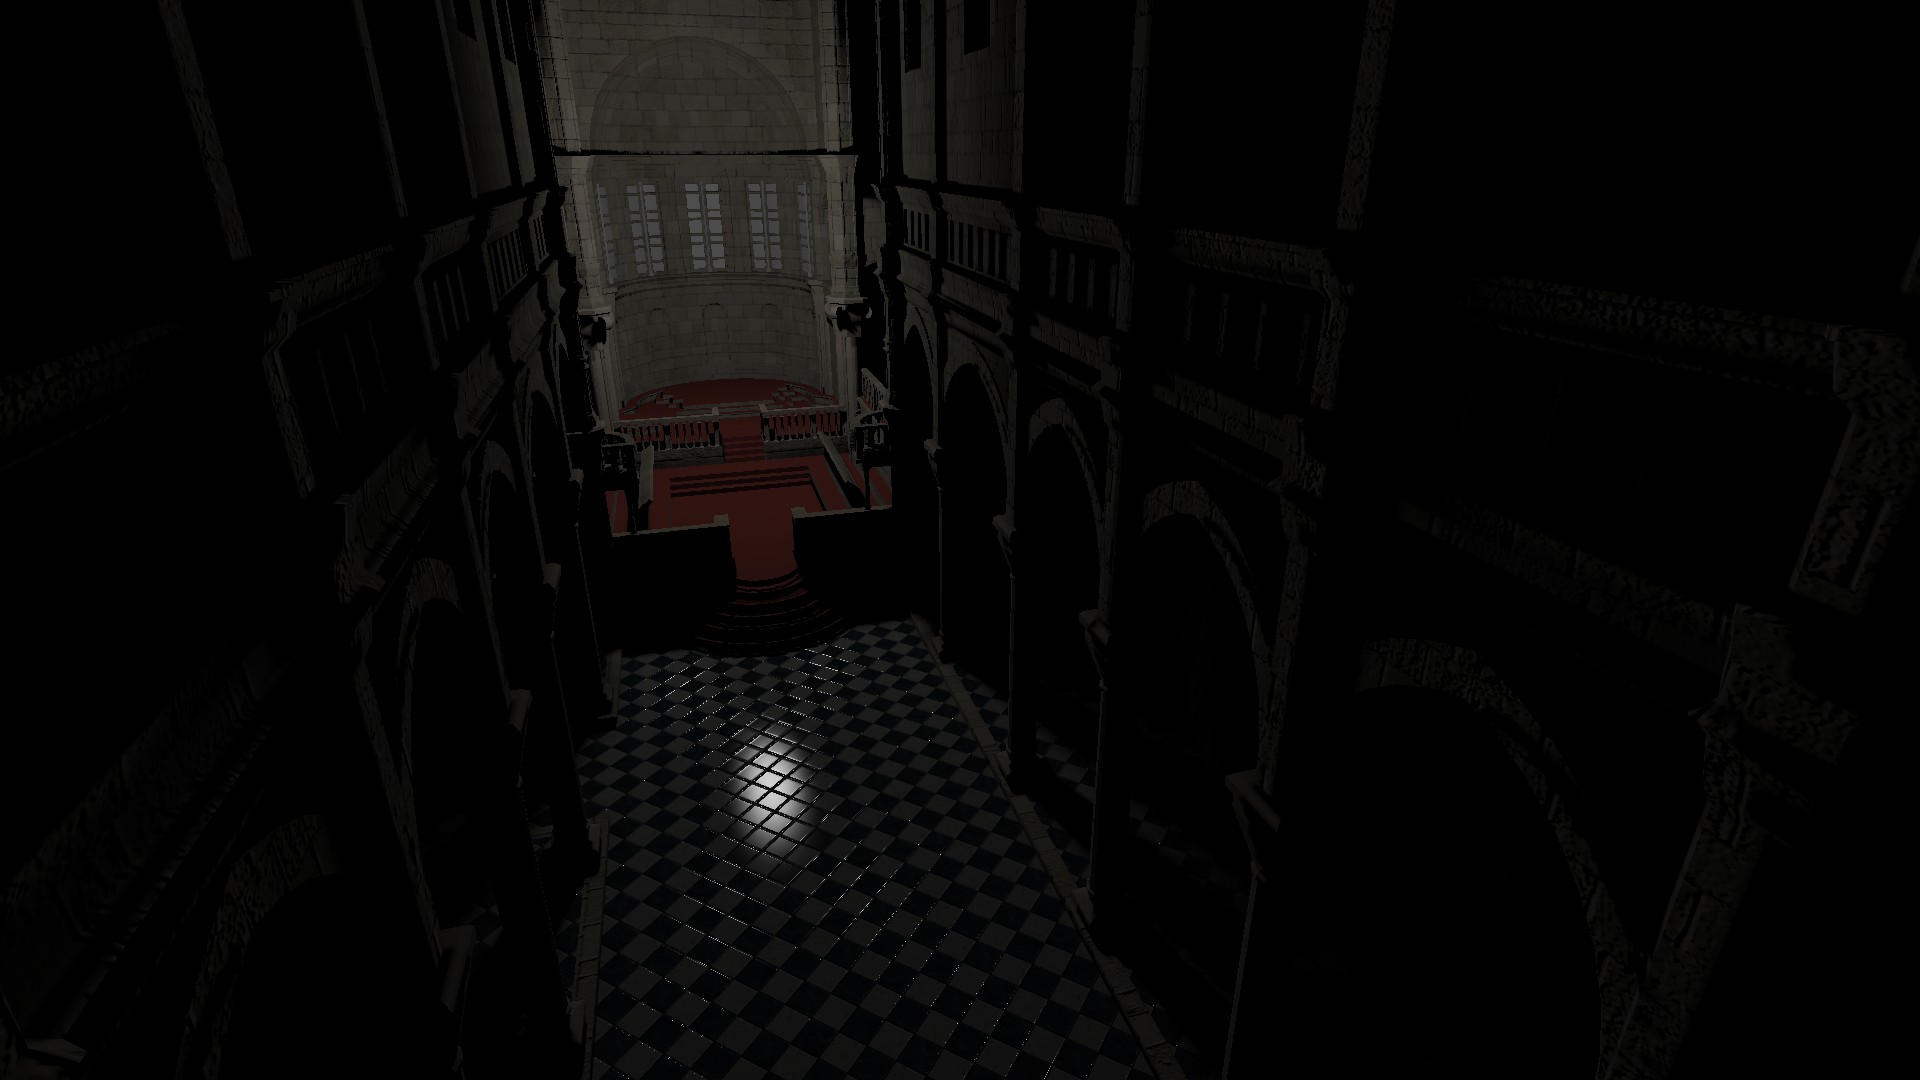
\includegraphics[width=\linewidth]{media/finals/sibenik_direct.png}
	\end{subfigure}%
	\hspace{0.01\textwidth}
	\begin{subfigure}[t]{.49\linewidth}
		\centering
		% \caption*{Indirecta}
		\captionsetup{justification=centering}
		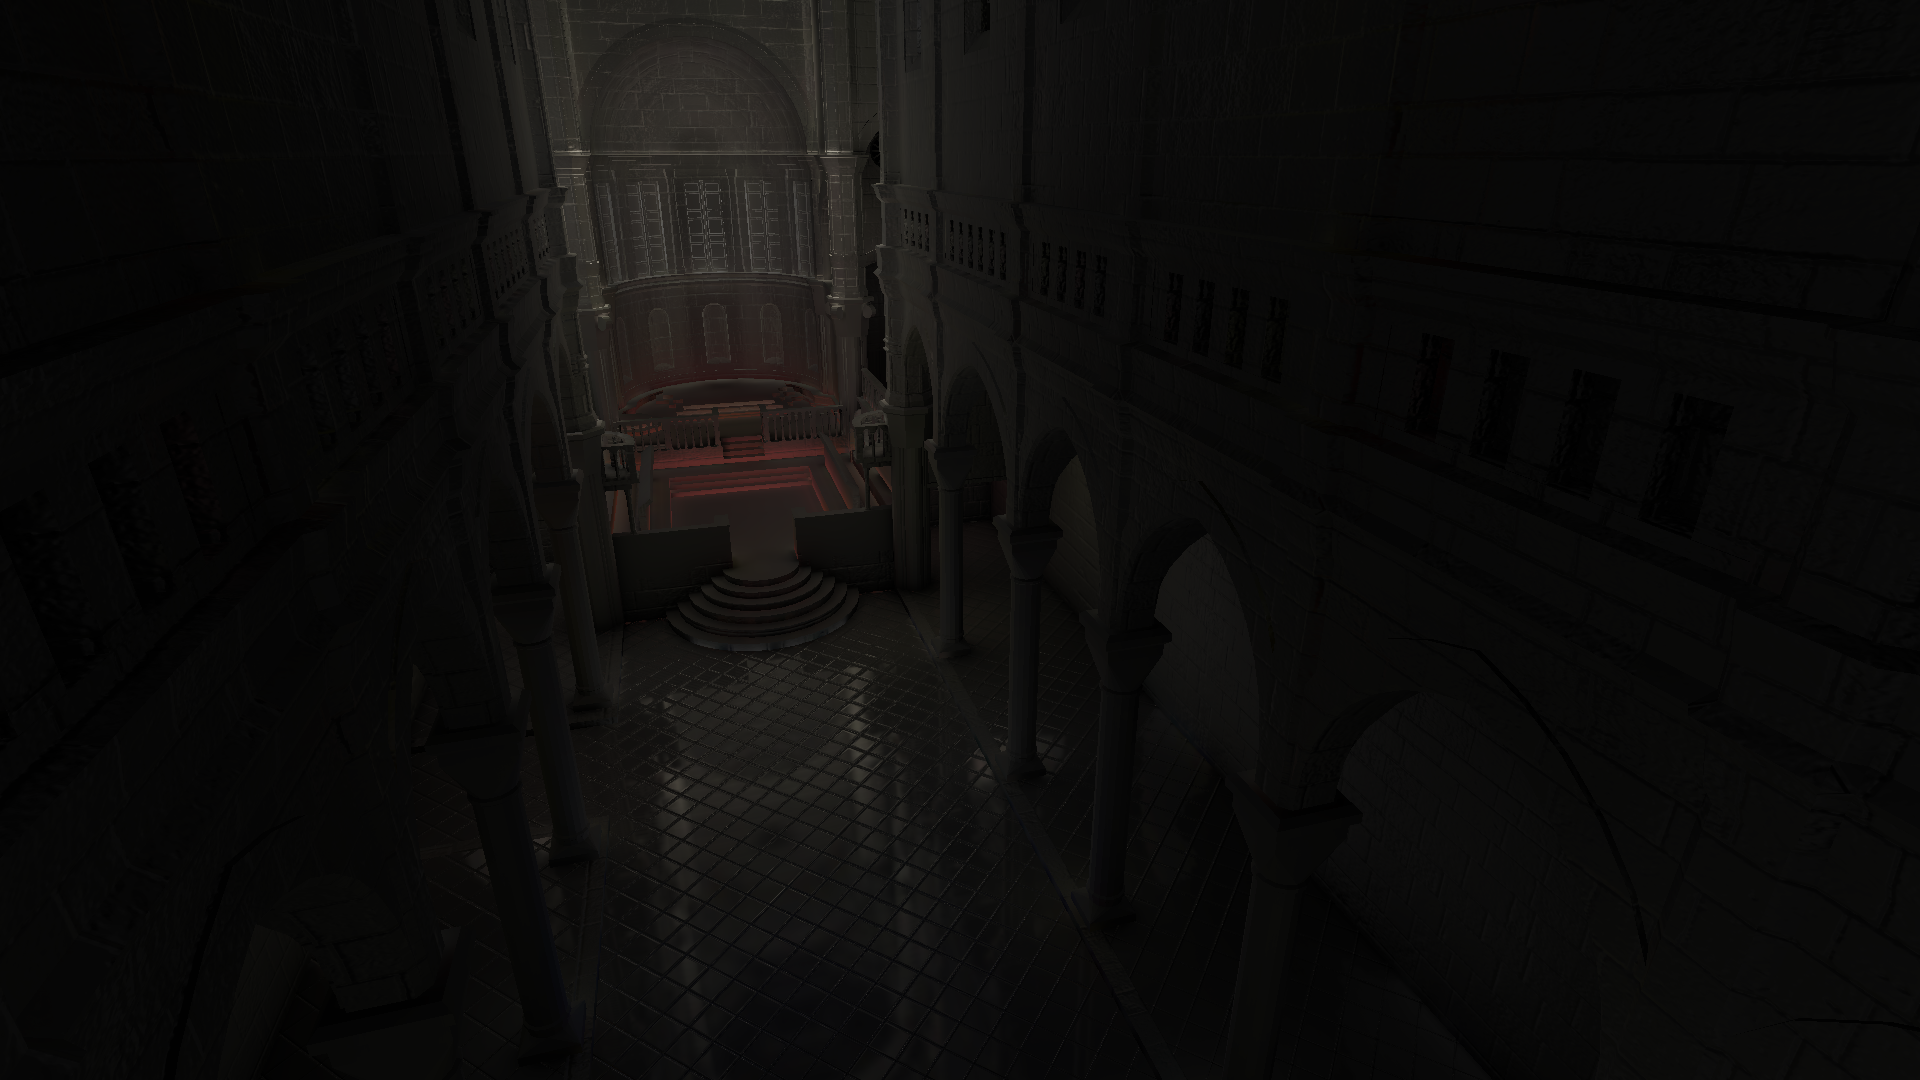
\includegraphics[width=\linewidth]{media/finals/sibenik_indirect.png}
	\end{subfigure}%
	\par\bigskip
	\begin{subfigure}[t]{.49\linewidth}
		\centering
		% \caption*{Directa + Indirecta + Oclusion Ambiental}
		\captionsetup{justification=centering}
		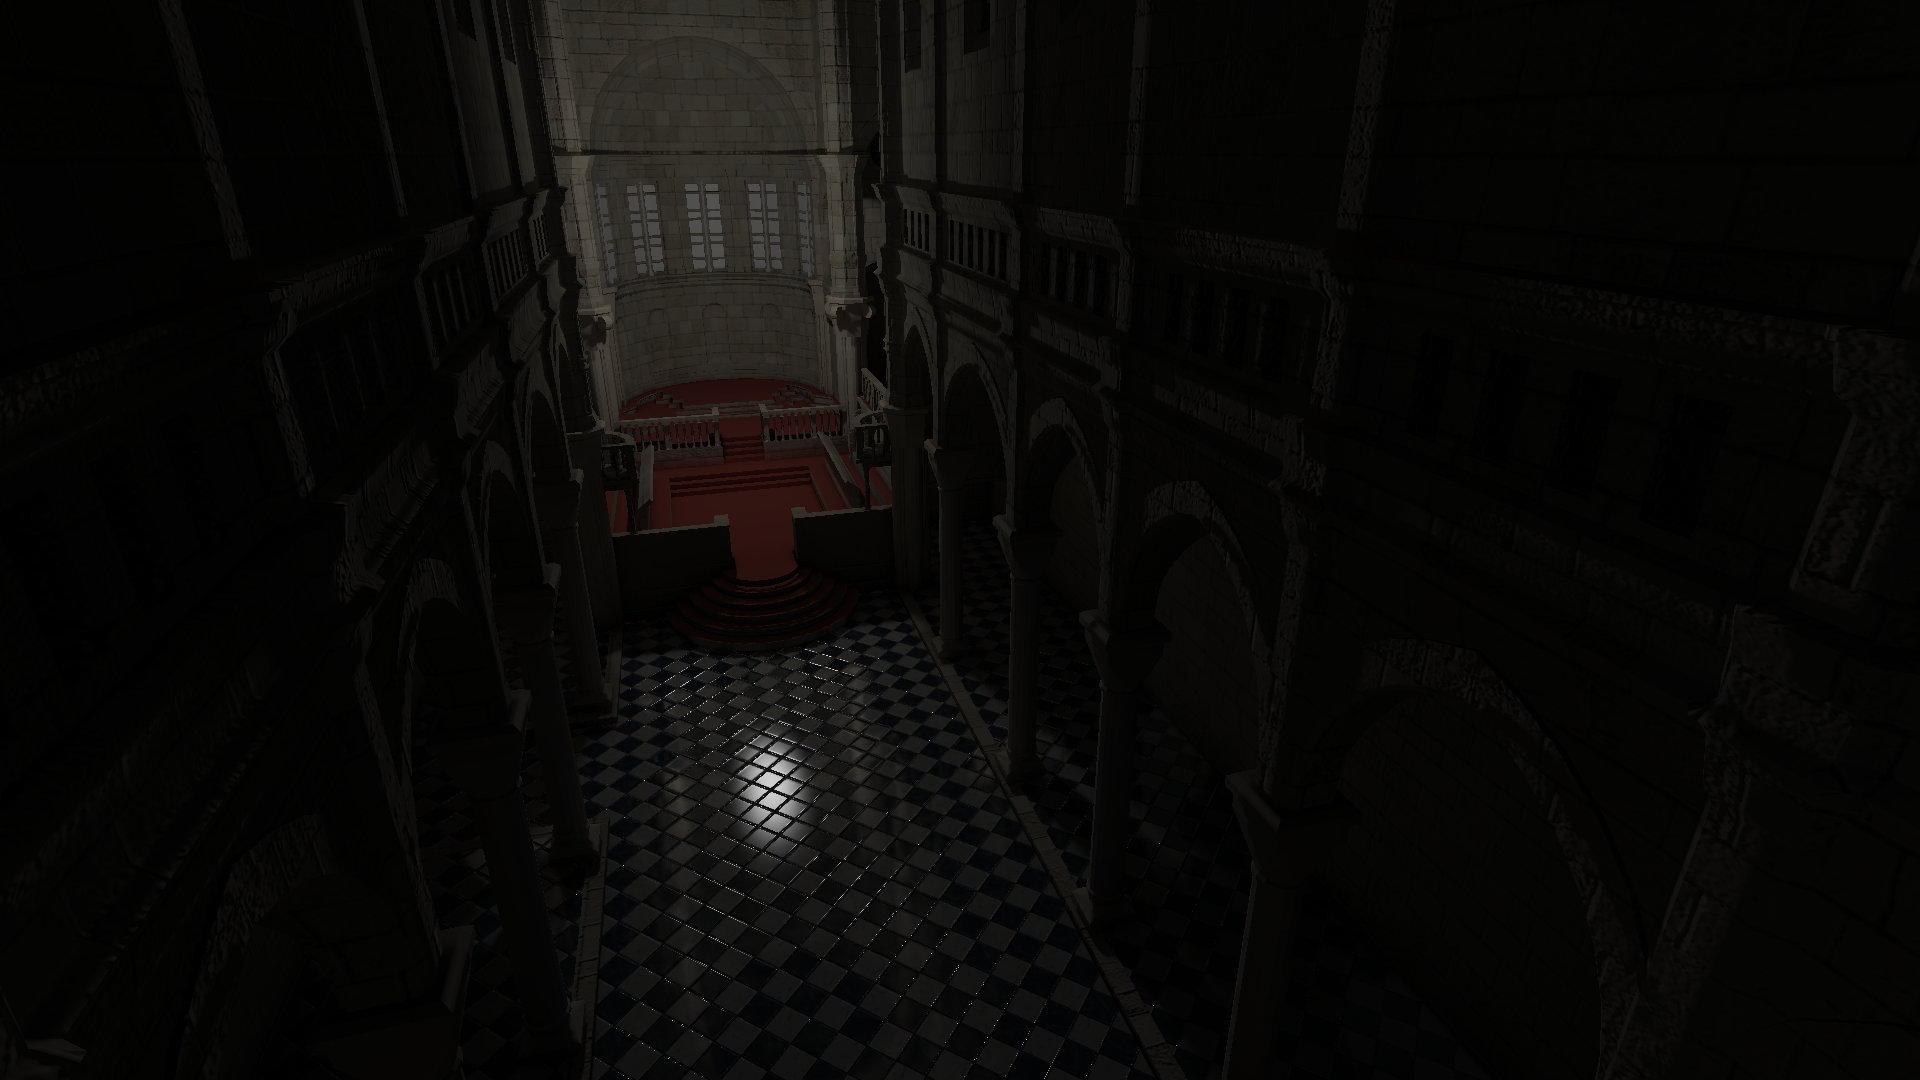
\includegraphics[width=\linewidth]{media/finals/sibenik_gi.png}
	\end{subfigure}%
	\hspace{0.01\textwidth}
	\begin{subfigure}[t]{.49\linewidth}
		\centering
		% \caption*{Oclusion Ambiental}
		\captionsetup{justification=centering}
		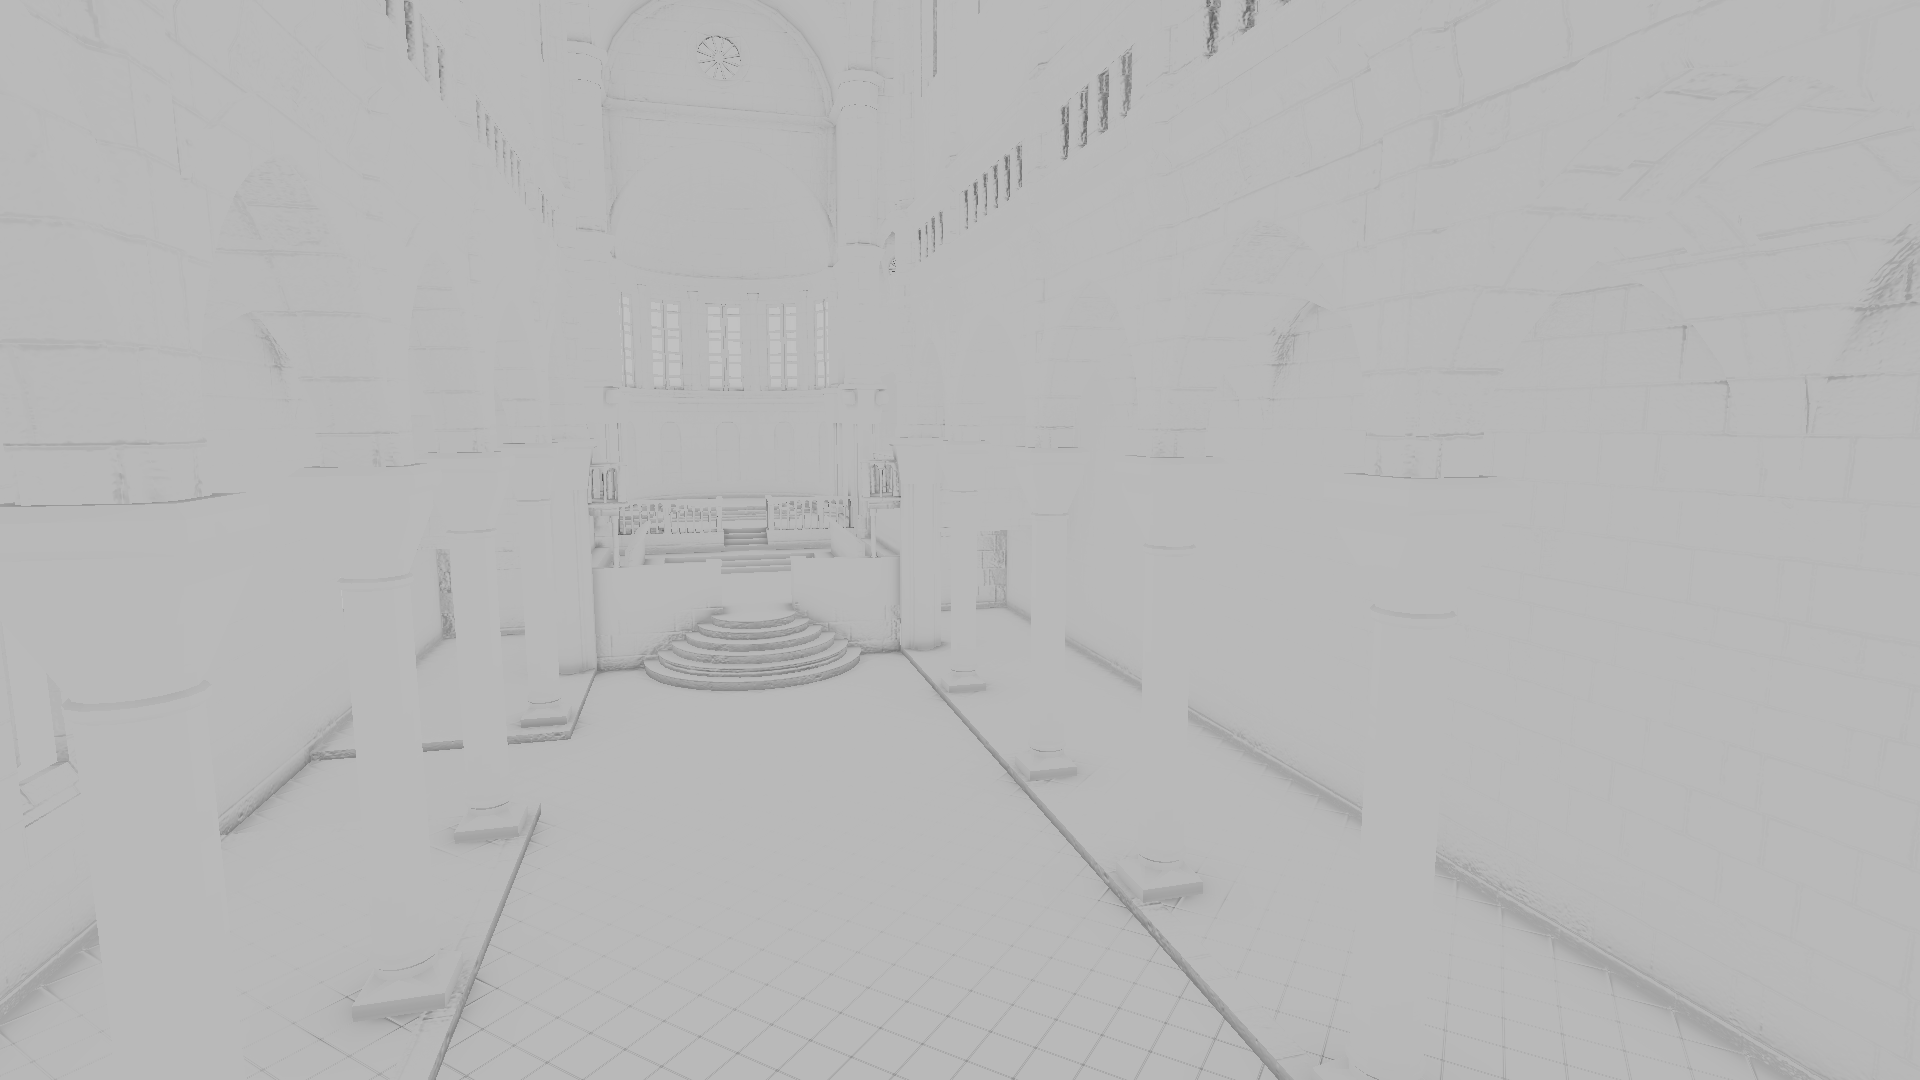
\includegraphics[width=\linewidth]{media/finals/sibenik_ao.png}
	\end{subfigure}%
	\caption{Composicion para la escena Sibenik.}
	\label{fig:sibenik_final}
\end{figure}
\begin{figure}[H]
	\centering
	\begin{subfigure}[t]{.49\linewidth}
		\centering
		\captionsetup{justification=centering}
		% \caption*{Directa}
		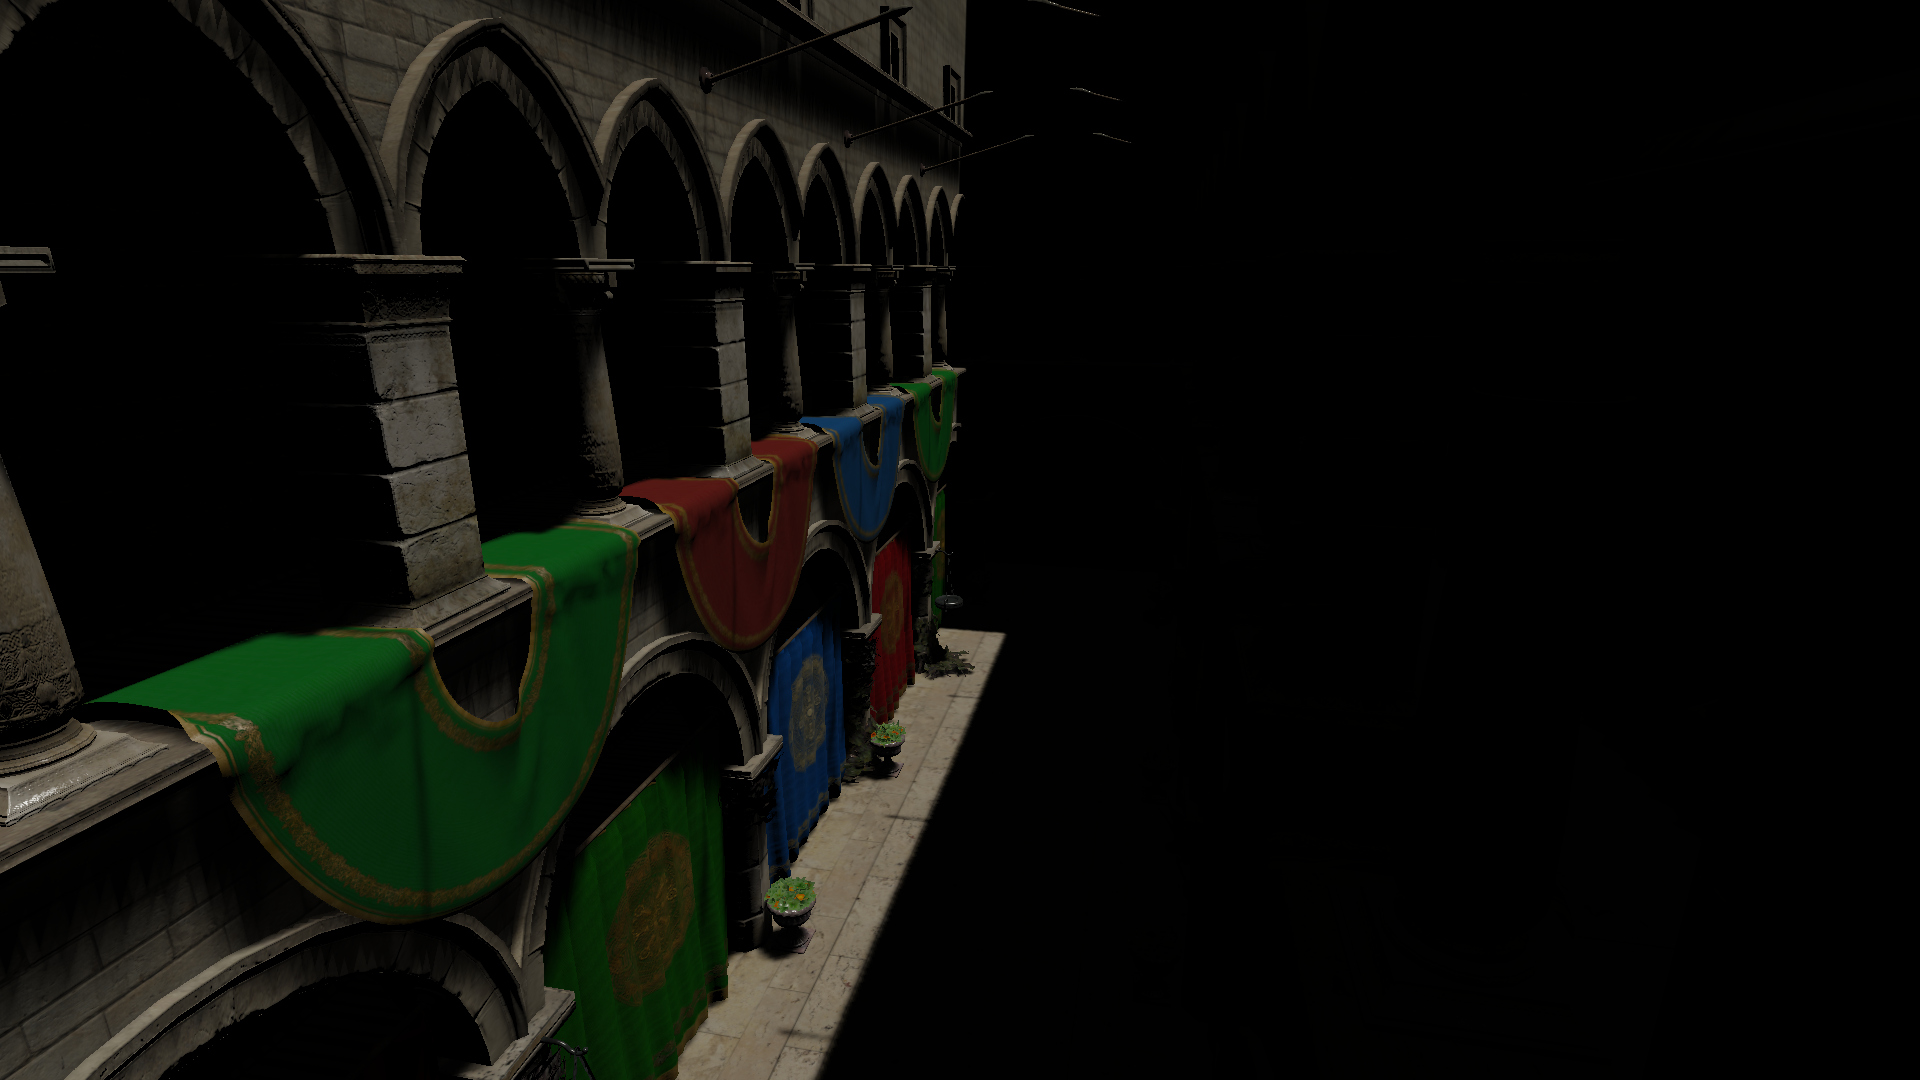
\includegraphics[width=\linewidth]{media/finals/sponza_direct.png}
	\end{subfigure}%
	\hspace{0.01\textwidth}
	\begin{subfigure}[t]{.49\linewidth}
		\centering
		% \caption*{Indirecta}
		\captionsetup{justification=centering}
		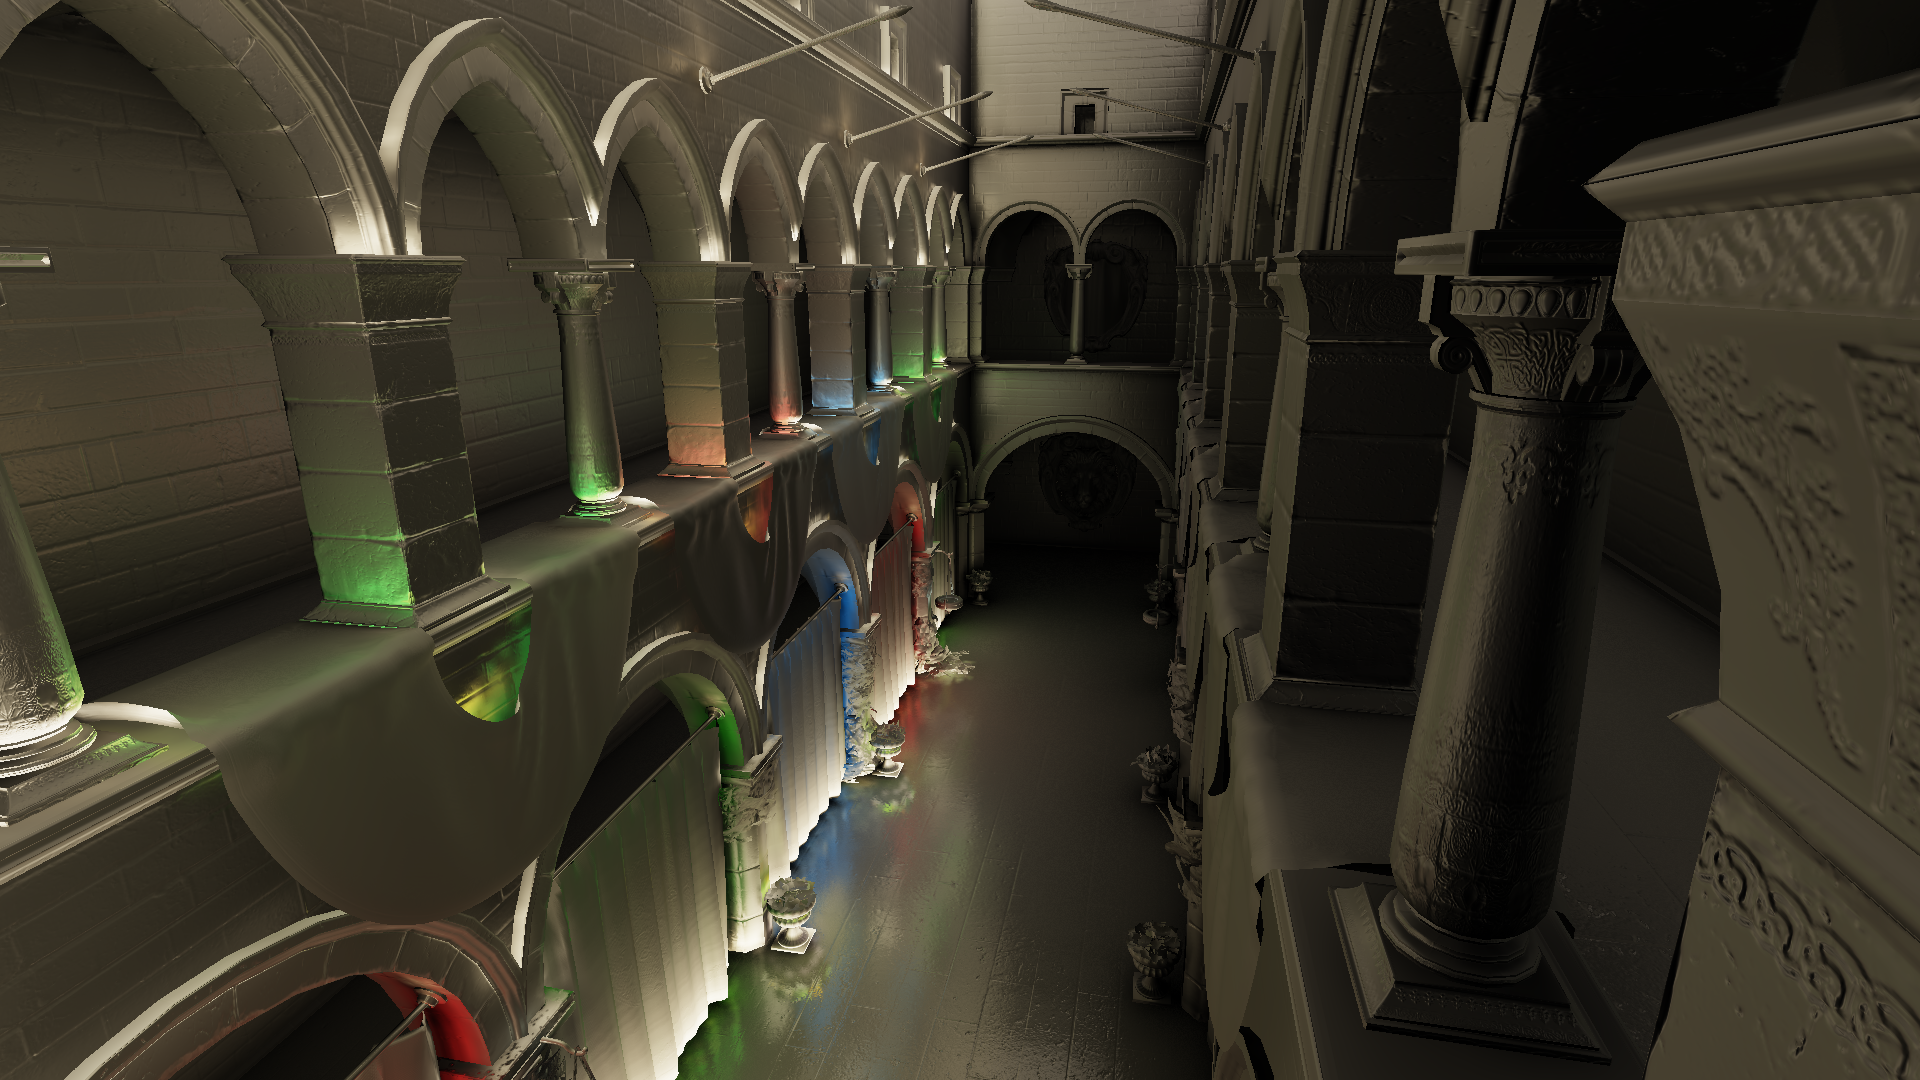
\includegraphics[width=\linewidth]{media/finals/sponza_indirect.png}
	\end{subfigure}%
	\par\bigskip
	\begin{subfigure}[t]{.49\linewidth}
		\centering
		% \caption*{Directa + Indirecta + Oclusion Ambiental}
		\captionsetup{justification=centering}
		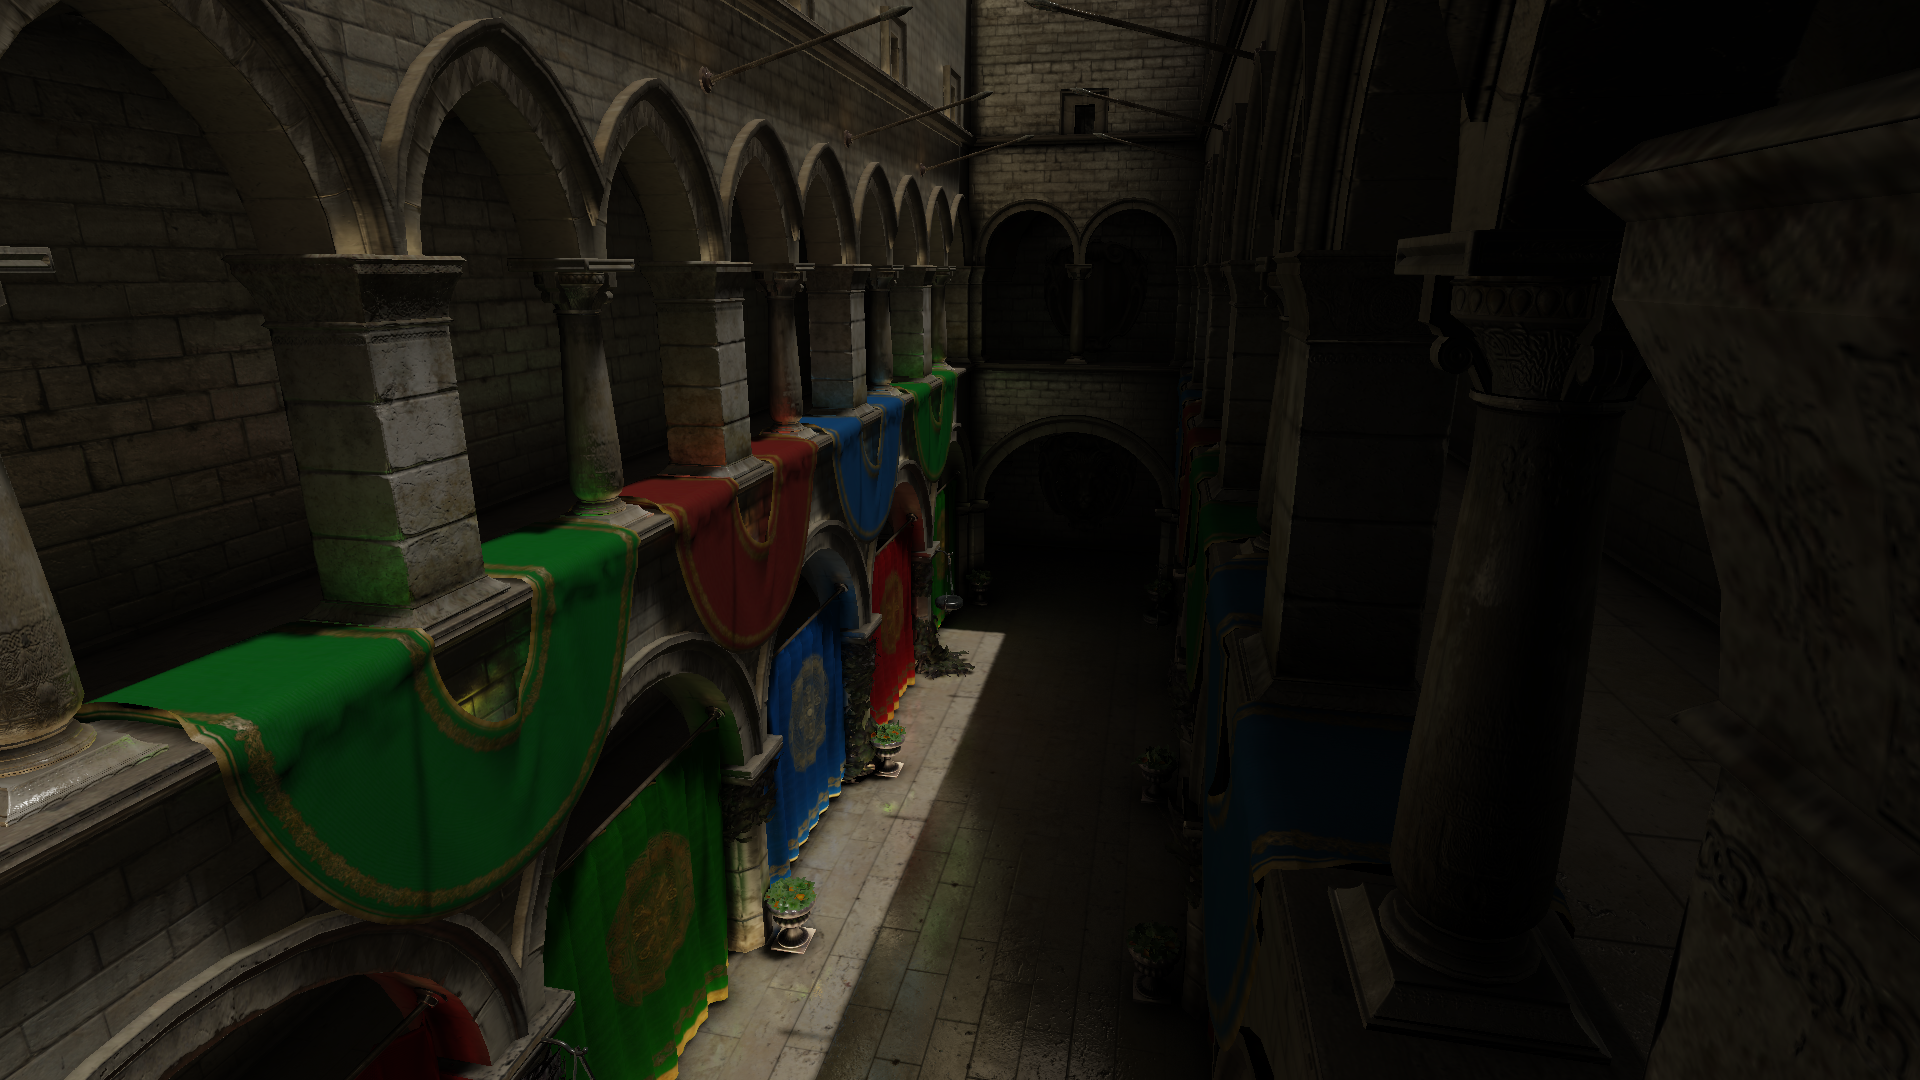
\includegraphics[width=\linewidth]{media/finals/sponza_gi.png}
	\end{subfigure}%
	\hspace{0.01\textwidth}
	\begin{subfigure}[t]{.49\linewidth}
		\centering
		% \caption*{Oclusion Ambiental}
		\captionsetup{justification=centering}
		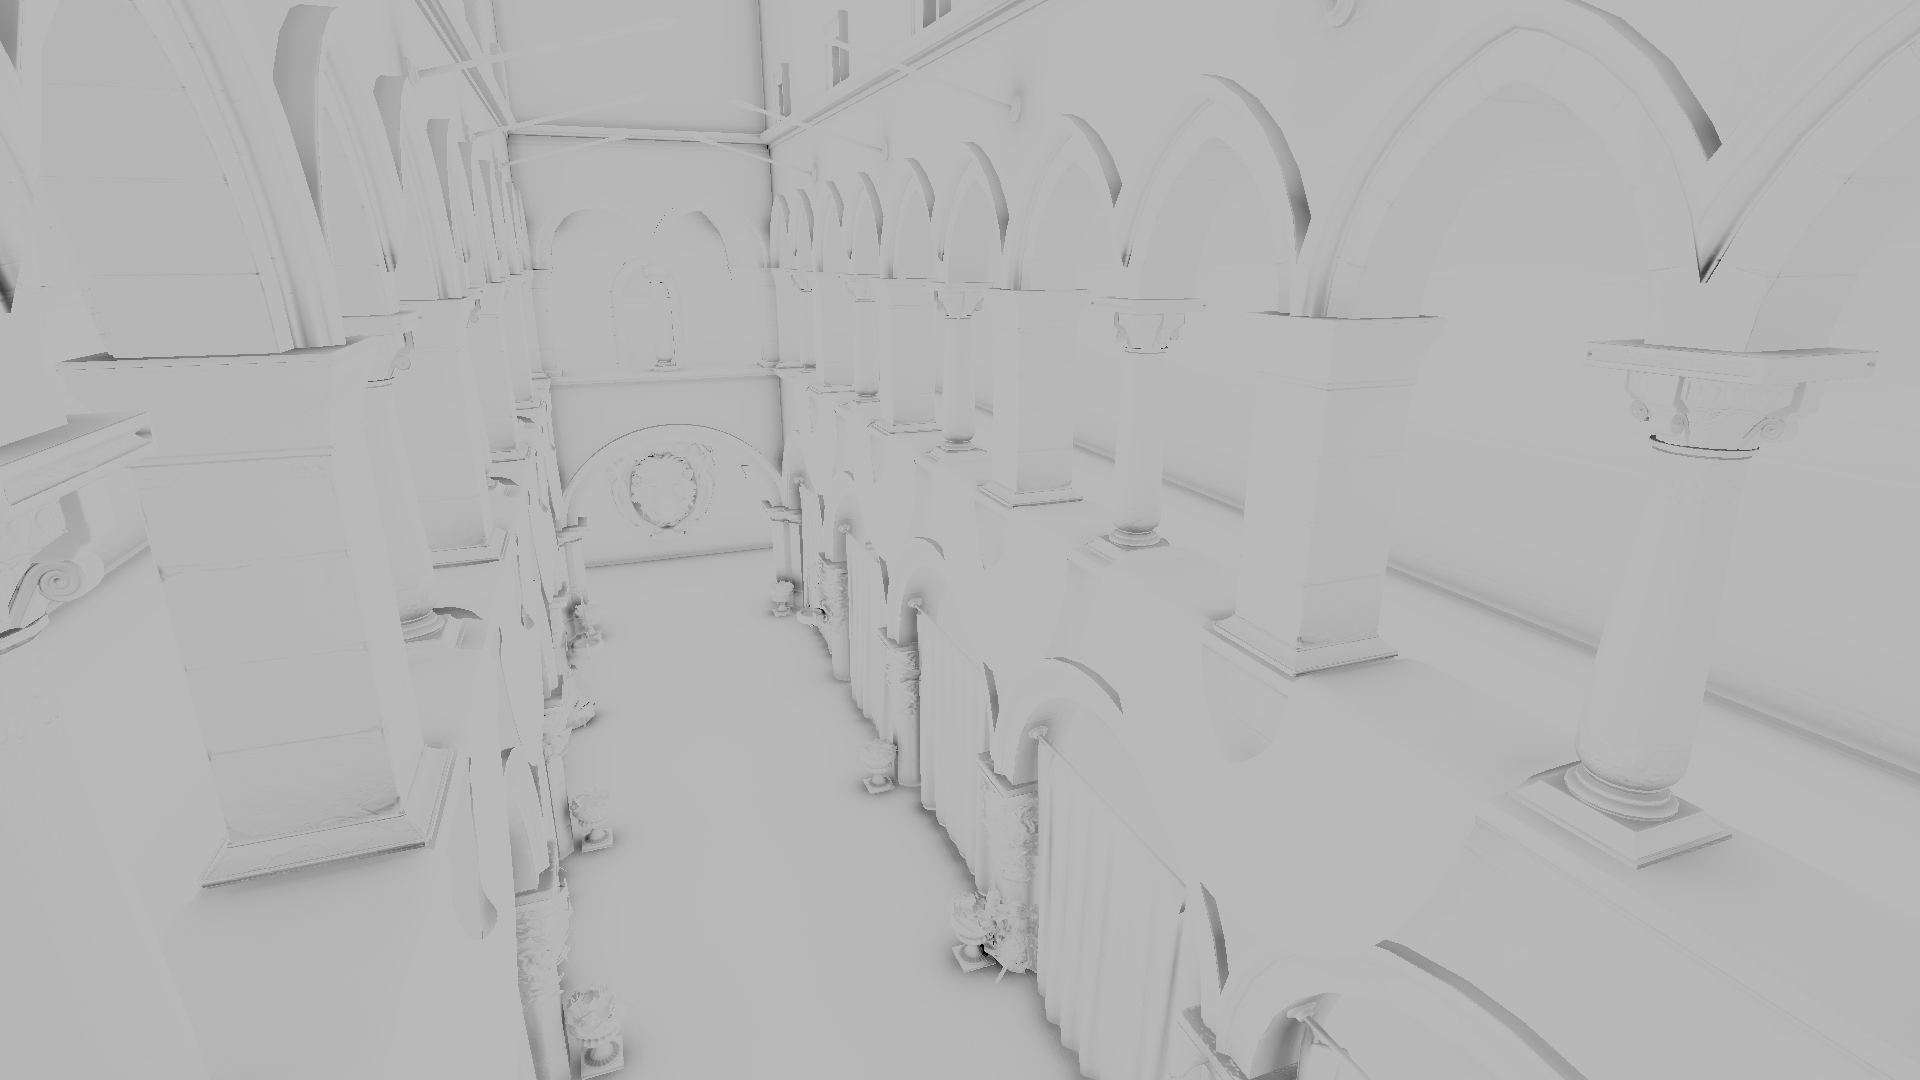
\includegraphics[width=\linewidth]{media/finals/sponza_ao.png}
	\end{subfigure}%
	\caption{Composicion para la escena Sponza.}
	\label{fig:sponza_final}
\end{figure}

\subsubsection{Iluminacion Global de Voxeles.}

